\chapter{Lecture 4 - Newton's Method and Secant Method}
\label{ch:lec4n}
\section{Objectives}
The objectives of this lecture are to:
\begin{itemize}
\item Describe and demonstrate Newton's method for solving non-linear equations.
\item Illustrate the convergence properties of Newton's method and highlight convergence issues.
\item Introduce and demonstrate the secant method.
\end{itemize}
\setcounter{lstannotation}{0}

\section{Introduction}
The bisection method described in the previous lecture had at least two issues:
\begin{enumerate}
\item End-points for the bracket $\left[a,b\right]$ in which a root is contained needed to be determined.  There is no cut-and-dried sure-fire way to accomplish this task.  Luckily, a suitable bracket can often be found even if such a method is hard to automate and may feel a bit ``clunky.''

\item The convergence rate is ``slow''---although we have not yet described any competing methods that are ``faster'' such that a proper perspective can be established.
\end{enumerate}
The open methods to be described in this lecture eliminate the first drawback of bracketing methods; open methods need no bracket containing a root, only an initial starting point.  Also, it will be shown, that the open methods described in this note converge more quickly than bracketing methods such as the bisection algorithm thereby clarifying the impact of the second drawback. 

On the other hand, open methods will introduce additional complications that offset some of their advantages.  These issues will be described and options for mitigating these complications will be presented.

\section{Newton's Method}

\begin{marginfigure}
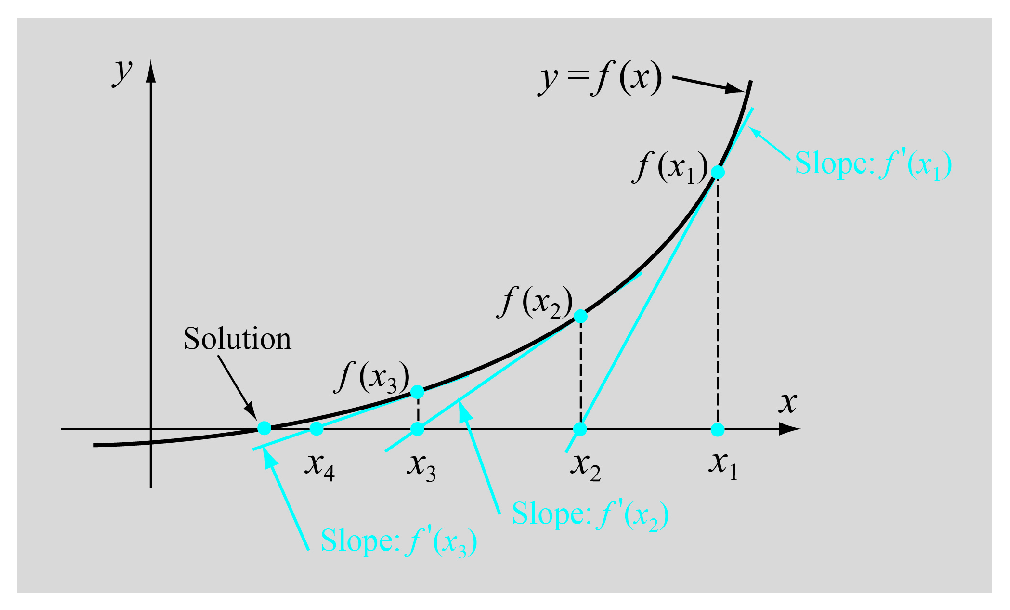
\includegraphics{Chapter3_Fig3_10.eps}
\caption{The first four iterations of Newton's method.}
\label{fig:newton-schematic}
\end{marginfigure}
Newton's method, also called the Newton-Raphson method, is a classic method for finding roots of equations that are \emph{continuous} and \emph{differentiable}. Given an initial estimate of the solution $x_1$, the second estimate is determined by taking the tangent line to $f(x)$ at the point $[x_1,f(x_1)]$ and finding the intersection of the tangent line with the $x$-axis. A schematic of the first four iterations of Newton's method is shown in Figure \ref{fig:newton-schematic}.  Successive estimates are found in the same way.  The slope of the tangent line at $x_1$ is denoted $f^{\prime}(x_1)$.  The point $x_2$ is determined from Equation \ref{eq:lec4n-newton-update}.\marginnote{\textbf{Note:} The expression for $x_2$ given in Equation \ref{eq:lec4n-newton-update} is obtained from: 

$$ f^{\prime}(x_1) = \frac{f(x_1)-0}{x_1 - x_2}$$
}
\begin{equation}
x_2 = x_1 - \frac{f(x_1)}{f^{\prime}(x_1)}
\label{eq:lec4n-newton-update}
\end{equation}
This process can ge generalized for finding solutions $x_{i+1}$ from $x_i$ as shown in Equation \ref{eq:lec4n-newton-update2}.
\begin{equation}
x_{i+1} = x_{i} - \frac{f(x_i)}{f^{\prime}(x_i)}
\label{eq:lec4n-newton-update2}
\end{equation}
The algorithm for Newton's method can be states as follows:
\begin{enumerate}
\item Choose a point $x_1$ as an initial guess of the solution.
\item For $i = 1,2,\dots,$ until the error is smaller than a specified tolerance, use Equation \ref{eq:lec4n-newton-update2} to find $x_{i+1}$ and repeat.
\end{enumerate}


\newthought{Since this is not} a bracketing method, we do not have a ``bracket'' to use in estimating the solution error like we did in the bisection method.  There are a couple of stopping criteria that could be used:
\begin{enumerate}
\item Tolerance in $f(x)$.  Recall from the last lecture, this means we will stop the iteration when, for some specified tolerance $\delta$, the following relation is satisfied:
\begin{equation}
\left| f(x_i) \right| \le \delta
\end{equation}
On the surface this is a sensible error measure---if $f(x_i)$ is close to zero, then it stands to reason that $x_i$ is close to the exact solution, $x^{\star}$.  It turns out, however, this is only true if $f^{\prime}(x_i) \approx 1$ in the vicinity of $x^{\star}$.  To see why, consider the equation below:
\begin{align*}
f^{\prime}(x_i) &\approx \frac{\cancelto{0}{f(x^{\star})}-f(x_i)}{x^{\star}-x_i} \\
\Rightarrow x^{\star} - x_i &\approx \frac{-f(x_i)}{f^{\prime}(x_i)}
\end{align*}
If $f^{\prime}(x_i) \approx 1$, then $|x^{\star} - x_{i}| \approx |f(x_i)| \le \delta$ which is what we want.  But if $f^{\prime}(x_{i}) < < 1$, then $|x^{\star} - x_{i}|$ is much greater than $\delta$ so we are not as close to $x^{\star}$ as we want to be.\sidenote{Remember that:
$$ x^{\star} - x_i = \frac{-f(x_i)}{f^{\prime}(x_i)}$$
Thus, as $f^{\prime}(x_i) \to 0$, then $x^{\star} - x_i \to \infty$.  }

\item Estimated relative error.  For Newton's method we will use the \emph{estimated relative error} as our measure of convergence.  Specifically, the iterations will be stopped when, for some specified tolerance $\epsilon$, the following relation is met:
\begin{equation}
\left|\frac{x_{i+1} - x_i}{x_i} \right| \le \epsilon
\end{equation}

\end{enumerate}

\section{Convergence Rate of Newton's Method}
To help illustrate the convergence rate of Newton's method, let us do an example.  We will find the positive root of the function: $f(x) = x^2 - 2$, which we know is equal to $\sqrt{2}$.  MATLAB code to implement the algorithm is shown in the listing below:
\marginnote{

\vspace{2.0cm}

\ref{lst:ann4n-1} We implement $f(x) = x^2-2$ and its derivative as in-line functions.

\vspace{0.25cm}

\ref{lst:ann4n-2} We do not need an initial bracket but we do need an initial guess.  For some problems it may be essential that the initial guess is close to the solution.

\vspace{0.5cm}

\ref{lst:ann4n-3} We will use the value of $\sqrt{2}$ to full double-precision to approximate the ``exact solution.''

}
\begin{lstlisting}[name=lec4n-ex1, style=myMatlab]
clear
clc
close 'all'

% find the square root of two
F = @(x) x.^2 - 2; /*!\annotation{lst:ann4n-1}!*/
dF = @(x) 2*x;

Xest = 1.; % initial guess /*!\annotation{lst:ann4n-2}!*/

Err = 1e-15;
imax = 5;
fprintf('Exact solution  = %16.15f \n',sqrt(2));/*!\annotation{lst:ann4n-3}!*/

for i = 1:imax
   Xi = Xest - F(Xest)/dF(Xest); 
    
   if abs((Xi - Xest)/Xest) < Err
       xNS = Xi;
       break;
   end
   
   fprintf('After %i iterations, Xi = %16.15f \n',i,Xi);
   
   Xest = Xi;      
end
\end{lstlisting}

An assessment of the output is shown below with the correct digits of the estimates solution shown in bold:
\begin{align*}
\sqrt{2} &\approx 1.414213562373095 \\
x_1 &= \mathbf{1.}500000000000000 \\
x_2 &= \mathbf{1.41}6666666666667 \\
x_3 &= \mathbf{1.41421}5686274510 \\
x_4 &= \mathbf{1.41421356237}4690 \\
x_5 &= \mathbf{1.414213562373095} 
\end{align*}
Note that between iteration 2 and 3, and between iteration 3 and 4, the number of correct digits doubles each time.  By the time that the 5th iteration is arrived at, the estimated solution is correct to full double precision.  It can be shown\cite{stewart1993afternotes} that the relative error in Newton's method can be approximated as:
\begin{equation*}
e_{i+1} \approx \frac{f^{\prime \prime}(x^{\star})}{2 f^{\prime}(x^{\star})}e_{i}^2
\end{equation*}
In words: the relative error at step $i+1$ is proportional to the error at step $i$ \emph{squared}.  This is referred to as \emph{quadratic convergence}.

\section{Convergence Issues with Newton's Method}
Alas, not all is well with Newton's method.  When the method works, it converges very rapidly.  Frequently, however, the method does not converge.  Convergence problems can happen under the following conditions:
\begin{enumerate}
\item When the value of $f^{\prime}(x)$ is close to zero in the vicinity of the solution.  When that happens, the update from $x_i$ to $x_{i+1}$ as given by Equation \ref{eq:lec4n-newton-update2} is very large.  If $x_i$ was close to the solution initially, $x_{i+1}$ may be very far from the solution.  Depending on how $f(x)$ varies between $x_i$ and $x_{i+1}$ this may result in convergence to a different root, for example, or other unpredictable behavior.

\item When the function has a local minimum (i.e. $f^{\prime} \approx 0$) in which case, again, the next iteration can be projected very far from the current value of $x_i$.  This condition is illustrated in Figure \ref{fig:lec4n-newton-troubles-a}.
\begin{marginfigure}[-4.0cm]
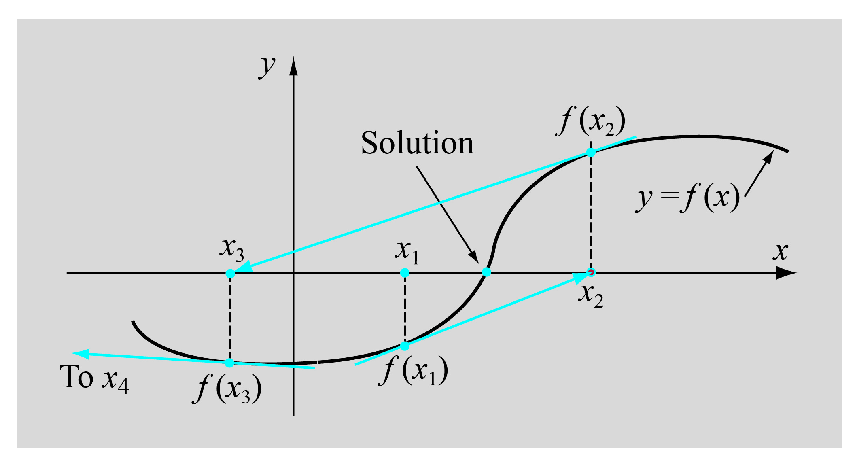
\includegraphics{Chapter3_Fig3_12a.eps}
\caption{Newton's method convergence issue due to a local minimum.}
\label{fig:lec4n-newton-troubles-a}
\end{marginfigure}

\item An inflection point can result in the iteration scheme entering into a cycle.  A schematic of this diabolical (and, thankfully, relatively uncommon) state of affairs is shown in Figure \ref{fig:lec4n-newton-troubles-b}.

\begin{marginfigure}
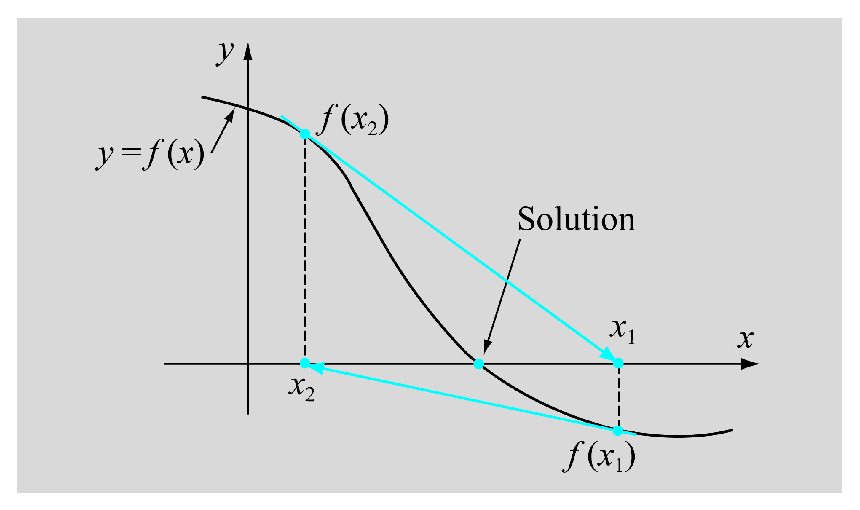
\includegraphics{Chapter3_Fig3_12b.eps}
\caption{Newton's method failure to converge due to inflection points in vicinity of solution.}
\label{fig:lec4n-newton-troubles-b}
\end{marginfigure}


\end{enumerate}
Notwithstanding these difficulties, it is possible to show that Newton's method will converge if the function, $f(x)$, and its first and second derivatives are all \emph{continuous}, and if the first derivative is not zero at the solution, and if the starting value, $x_1$, is ``near'' the exact solution.\sidenote{Whatever the hell ``near'' is supposed to mean.}

\newthought{Another issue with} Newton's method, not directly related to convergence, is that to use the method you need both the function as well as its derivative.  The derivative is not always easy to obtain.  In some cases the ``function'' to be solved is not available in the form of an equation but rather a complex computational routine that does not admit to analytical differentiation.  Combined with the convergence difficulties, there is plenty of motivation to come up with a different algorithm.

\section{Secant Method}
The secant method is another open scheme for finding a numerical solution to a non-linear equation.  Unlike Newton's method, the secant method does not require an expression for $f^{\prime}(x)$.  With the secant method we instead approximate this derivative by using the \emph{secant line} between \emph{two} initially provided points. This is illustrated in Figure \ref{fig:lec4n-secant-schematic} where it is also shown that it does not matter if $x_1$ and $x_2$ bracket the root or not.
\begin{figure}[h!]
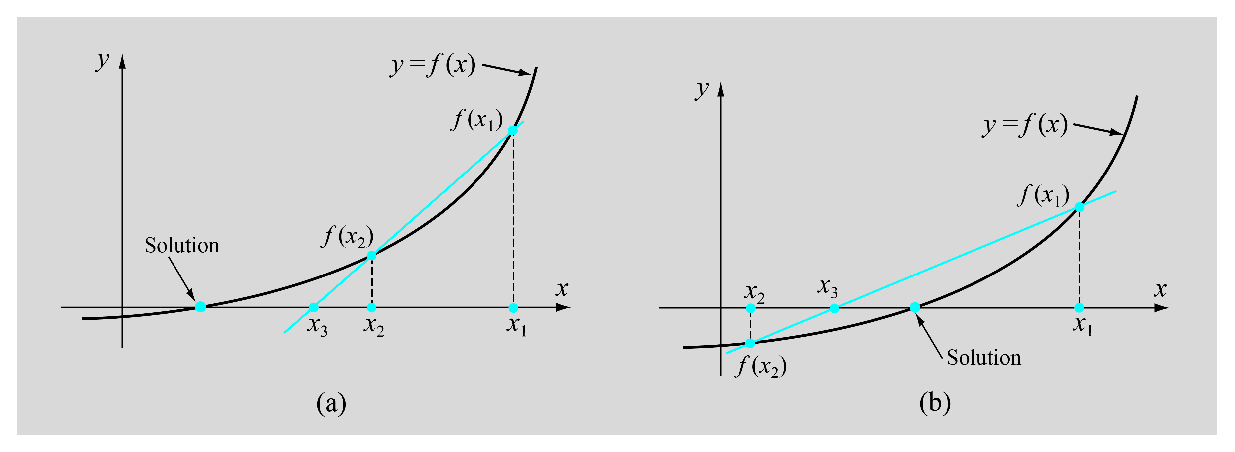
\includegraphics{Chapter3_Fig3_14.eps}
\caption{Schematic of the secant method.}
\label{fig:lec4n-secant-schematic}
\end{figure} 

\noindent The slope of the secant line is given by:
\begin{align*}
&\frac{f(x_1) - f(x_2)}{x_1 - x_2} = \frac{f(x_2) - 0}{x_2 - x_3} \\
& x_3 = x_2 - \frac{f(x_2)(x_1 - x_2)}{f(x_1)-f(x_2)}
\end{align*}
Once $x_3$ is determined, it is used along with $x_2$ to find $x_4$ and so it goes.  We generalize this iteration in Equation \ref{eq:secant-it}.\marginnote[-1.25cm]{\textbf{Note:} We can slightly re-arrange Equation \ref{eq:secant-it} to get:
$$ x_{i+1} = x_i - \frac{f(x_i)}{\frac{f(x_{i-1}) - f(x_i)}{(x_{i-1} - x_i)}}$$
This may help emphasize the similarity between the secant method and Newton's method.  If $x_{i-1}$ and $x_{i}$ are sufficiently close together:
$$\frac{f(x_{i-1})-f(x_i)}{x_{i-1}-x_i} \approx f^{\prime}(x_i)$$
}

\begin{equation}
x_{i+1} = x_i - \frac{f(x_i)(x_{i-1} - x_i)}{f(x_{i-1}) - f(x_i)}
\label{eq:secant-it}
\end{equation}
Successive iterations of the secant method are illustrated in Figure \ref{fig:lec4n-secant2}.
\begin{marginfigure}
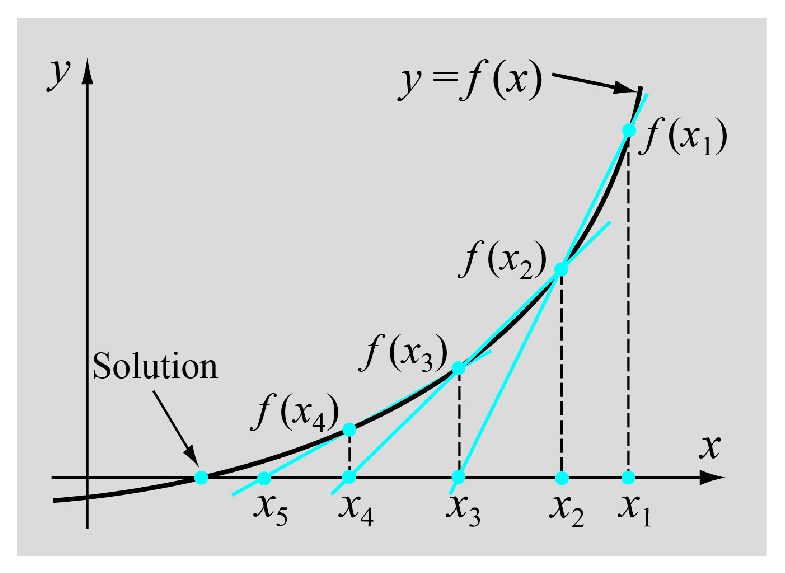
\includegraphics{Chapter3_Fig3_15.eps}
\caption{Secant method in action.}
\label{fig:lec4n-secant2}
\end{marginfigure}

\newthought{While the secant} method does not rely on an expression for $f^{\prime}(x)$, it does require additional evaluations of $f(x)$.  If each evaluation of $f(x)$ is computationally expensive then the programmer who is implementing the method would be wise to minimize or eliminate any extraneous evaluations of $f(x)$.  While this point probably seems obvious, it is worth mentioning that this consideration amounts to a design trade-off.  Program complexity and the number of additional variables that you may store to avoid re-evaluating a function can add up.  Sometimes it pays to simply re-compute $f(x)$ whenever you need it; sometimes it does not.  Keep this in mind when you design your own implementation.

\section{Convergence of Secant Method}
The MATLAB code for testing the convergence of the secant method is provided in the listing below. Again we solve the equation: $f(x) = x^2 - 2$.  We use the starting points, $x_1 = 0$ and $x_2 = 2$.

\begin{lstlisting}[name=lec4n-ex2, style=myMatlab]
clear
clc
close 'all'

% find the square root of two
F = @(x) x.^2 - 2;

Xa = 0; 
Xb = 2;

Err = 1e-16;
imax = 15;
fprintf('Exact solution = %16.15f \n',sqrt(2));
for i = 1:imax
   FXb = F(Xb);
   Xi = Xb - FXb*(Xa - Xb)/(F(Xa) - FXb);
   
   if abs((Xi - Xb)/Xb) < Err
       xNS = Xi;
       break;
   end
   Xa = Xb;
   Xb = Xi;
   
   fprintf('After %i iterations, Xi = %16.15f \n',i,Xi);          
end
\end{lstlisting}
Results are as shown below:
\begin{align*}
\sqrt{2} &\approx 1.414213562373095 \\
x_1 &= \mathbf{1.}000000000000000 \\
x_2 &= \mathbf{1.}333333333333333 \\
x_3 &= \mathbf{1.4}28571428571429 \\
x_4 &= \mathbf{1.41}3793103448276 \\
x_5 &= \mathbf{1.41421}1438474870 \\
x_6 &= \mathbf{1.414213562}688870 \\
x_7 &= \mathbf{1.414213562373095}
\end{align*}
Clearly the convergence rate for the secant method is inferior to Newton's method\sidenote{It should be noted that the exact convergence behavior depends, to some extent, on the values chosen for $x_1$ and $x_2$.} and yet, it is still better than bisection method.

\section{Wrap-up}
In this lecture we investigated open root-finding methods that, using the derivative of a function or, in the case of the secant method, an estimate of the derivative of a function, to find the root of a non-linear equation.  We found that, for the expense of using the derivative, or estimate of a derivative, of a function, we were able to get quadratic convergence.  If you need to get a very precise solution and/or individual function evaluations are computationally expensive, these methods have strong advantages over bisection.  

\newthought{There are at least} two questions that you should be asking yourself:
\begin{enumerate}
\item Can I get even faster convergence if I also make use of the \emph{second} derivative of the function?  The answer is: \textbf{yes}.  The algorithm that takes this approach is called Halley's method\cite{gander1985halley} and the error after each iteration is proportional to the error after the previous step \emph{cubed}.

\item Can I get convergence faster than the bisection method while retaining the reliability of the bisection method?  The answer is also \textbf{yes}.  The Brent method combines techniques based on the secant method, bisection method, and inverse quadratic interpolation to converge \emph{at least} as fast as bisection---often much faster---while retaining the robust reliability of bisection.  Theoretical details of the Brent method are available in the literature\cite{forsythe1977computer} and a straightforward example implementation is given in a popular Numerical Recipes\cite{press1988numerical} book.  MATLAB's built-in non-linear equation solver \lstinline[style=myMatlab]{fsolve} is based on Brent's method.

\end{enumerate}
Homework problems will be assigned that will help you explore the practical details of implementing these algorithms and observing the convergence properties.
